\documentclass[a4paper,10 pt]{article}
\usepackage{geometry}
\geometry{letterpaper, margin=0.8in}
\usepackage[english]{babel}
\usepackage[utf8]{inputenc}
\usepackage{amsmath}
\usepackage{graphicx}
\usepackage[colorinlistoftodos]{todonotes}
\usepackage{float}
\usepackage[numbered]{mcode}
\usepackage{minted}
\renewcommand{\baselinestretch}{1.1}

\title{Neural Networks for Image Recognition: Fashioning the Right Architecture}

\author{Dana Korssjoen} 

\date{13 March 2020}

\begin{document}
\maketitle
\begin{abstract}
    This report explores the use of fully-connected and convolutional neural networks for recognition on the fashion-MNIST dataset. Theoretical background on both architectures, design choices for this task, and computational results are discussed in their respective sections.
\end{abstract}
\section{Introduction and Overview}
Neural networks are very en vogue at the moment, particularly for computer vision tasks. It's fitting, then, that we explore the application and implementation of two classic networks, the fully-connected neural network and the convolutional network, on the fashion-MNIST dataset. The goal for both architectures in this report is simple: classify the images with as high accuracy as possible. This paper discusses the theoretical background of both architectures, as well as neural networks in general, in order to preface a discussion of design choices. In the following section, justification for algorithm implementation is made, and both architectures are developed. They are then evaluated and compared. Finally, we will discuss findings and their implications.

\section{Theoretical Background}
\subsection{Neural Networks}
As implied by the name, neural networks are a computational model motivated by the structure of biological neurons. The basic idea is that each artificial neuron in the network can take input, perform a simple computation, and output the result. So each individual neuron is quite simple but, just like in a human brain, when those neurons are combined and connected in large numbers, the network can perform extremely sophisticated tasks. 

There are many ways to connect artificial neurons in a neural network. The two major architecture explored in this report are fully connected networks, and convolutional networks. In both designs, neurons are arranged into layers which the data will proceed through sequentially. In a fully connected network, each neuron in a given layer is connected to every other neuron in the previous layer. In a convolutional network, this is not the case. We can think about a convolutional layer as shining a flashlight over the data, and letting the input of neuron $j$ be only those parts of the data that are illuminated when the flashlight is at position $j$. In other words, each neuron looks at only part of the data, and adjacent neurons look at adjacent parts.

Regardless of how you choose to connect layers of neurons, each individual connection between neurons can have its own weight. The optimal value for this weight is learning by the neural network during training, which is discussed later in this section. Each layer also adds some bias, which functions a lot like a weight.

Another way in which neural networks model the biological brain, is that individual neurons can be activated by their input. That is, we can give neurons activation functions which will determine if their input is sufficient to activate them. The activation function used in this report is LeakyReLU (Leaky Rectified Linear Unit), which is given by
\begin{equation}
    \sigma(x) = \max\{\alpha x, x\},\quad\quad 0<\alpha<1,
\end{equation}
which essentially is meant to give a negative value when the input is negative, likewise for positive, and to avoid the issue of vanishing gradients, which can be troublesome during backpropagation. 

Before we can dive into backpropagation, we need to discuss loss functions, which calculate the error of our model. A common loss function for classification tasks, and the one used in this report, is cross-entropy loss. To calculate this loss, say that we have $K$ total classes and we know that observation $j$ belongs to class $k$. Mathematically, we say that $y_j$ is a one-hot vector with entry 1 in position $k$. Now, if our model calculates that the probability that observation $j$ belongs to class $k$ is $p_j$, then cross-entropy loss is given by
\begin{equation}
    L = -\frac{1}{N}\sum_{j=1}^N \ln(p_j),
\end{equation}
where $N$ is the total number of data points. The reason why we take the log of $p_j$ is because we want to make sure our function will be convex, or else we will run into all sorts of problems during training. Moreover, we can actually regularize this function by adding a term to the loss function, as in 
\begin{equation}
    L = -\frac{1}{N}\sum_{j=1}^N \ln(p_j) + \lambda ||\mathbf{w}||_2^2,
\end{equation}
which prevents the weights from getting too large, preventing overfitting. In this equation, $\lambda$ is the regularization parameter. 

To train the network, we want to find the weights and biases that minimize our loss function. To do this, we need an optimization algorithm. The algorithm used in this analysis is Adam, which is short for adaptive moment estimation. Adam is an extension of mini-batch gradient descent that adapts its parameter learning rates as it trains. Specifically, the core idea is mini-batch gradient descent, which is a gradient descent algorithm that only runs on a subset of the data (the ``batch'') at any given time, which decreases computational complexity compared to full-batch gradient descent. Adam innovates on this idea by adapting the learning rate for different parameters based on the mean and variance of the gradient at that time.

Regardless of which optimization function is chosen, the network needs to get updated with the new weights and biases. This is done via backpropagation, meaning that we update the parameters for the last layer first, then use those values to update the layer before it, etc. until we get to the first layer and we've finished updating the network. The reason why we work ``backwards'' like this is because in a sequential network, each parameter affects the parameters in front of it, but parameters don't affect the ones behind them. So when we change the very last value in the ``chain'' of neurons, we can isolate for the effect that change will have on the overall output, then work backwards.

Armed with this background, we are ready for implementation.

\section{Algorithm Implementation and Development}
\subsection{Load and Prepare the Data}
We see this on lines 1 - 17 and 61 - 77. There's nothing fancy here; we're just loading the necessary packages, plus the dataset, then reserving the first 5000 entries of the training set for validation. We'll use these to experiment with different hyperparameters. We divide by 255.0 to convert each of our pixels into a float from $[0,1]$.

\subsection{Build the Model, Part I: Fully Connected Architecture}
We see this on lines 19 - 41. The activation function used in all of the internal layers of this network will be LeakyReLU, which has the advantages discussed in the Theoretical Background section. Several other activation functions, including ReLU and tanh, were tested, but this was found to be the best choice. A simple 2-norm regularizer was added to prevent overfitting, since we'll be training this over quite a few epochs, and we don't want to overfit. In between layers, we perform batch normalization, so that the input to each layer comes from a normal distribution. Finally, the last layer uses a softmax activation so that we can get probabilities (summing to 1) of the input belonging to each of the 10 classes.

The choices for loss function (cross-entropy) and optimizer (Adam) are discussed in the Theoretical Background section. The learning rate was chosen experimentally.

\subsection{Build the Model, Part II: Convolutional Architecture}
We see this on lines 79 - 102. As before, LeakyReLU is used on the fully connected layers, as is a small 2-norm regularizer. For the convolutional layers, many parameters were adjusted experimentally. In particular, MaxPooling and AveragePooling were compared, with MaxPooling performing significantly better with a range of filter sizes. Other major design choices were same padding and stride values. Again, softmax is used for activating the final layer to get the output to have the desired attributes. The choices for loss function and optimizer are as in Part I. Learning rate was edited experimentally, but the value chosen here (0.0001) resulted in the best performance.

\subsection{Evaluate the Model}
We see this on lines 44 - 58 and 104 - 118. Here, we simply see how the model performs on data that it has never seen before (the testing data). It outputs the accuracy rate mentioned in the Computational Results section. We also plot how the accuracy and loss changed as the training epochs progressed, and we compute and save the confusion matrix. These results are included in the next section.

\section{Computational Results}
This section discusses the results of the fully-connected (or dense) network, and the convolutional neural network (or CNN). In figures 1 and 3, we can see the training progress of the dense network and CNN, respectively. In both, we see that the accuracy on both the training and validation data increase relatively monotonically throughout training. We stop at the point that the progress seems to level off. Note that we should start to worry about overtraining once the validation accuracy begins to decline, which doesn't happen in either case, so overtraining shouldn't be a big issue here. In fact, it wasn't; on the test data, the dense network had an accuracy rate of $0.8913$ (or 89.13\%), and the CNN had a rate of $0.9193$ (or 91.93\%). These are roughly equivalent to their end validation accuracies, at $0.8970$ and $0.9214$, respectively.

Overall, the CNN performed better than the dense network throughout training, as well as during testing. So in general, we can say that the CNN was more accurate. If we want to compare the networks on a more granular level, we can take a look at their confusion matrices in figures 2 and 4. The rows of the matrix correspond to actual data classes, the columns correspond to predicted classes, and the entries correspond to how many of that combination there are. Concretely, when you see the number 4 in row 2, column 0 of figure 2, it means that the model thought that a true 2 was a 0 exactly 4 times in the testing data.

From the confusion matrices, we can make an interesting observation; the networks struggled with different pairs of numbers. Specifically, the dense network most often mistook 0s for 6s (103 times), 6s for 0s (96 times), and 2s for 6s (64 times); for the CNN, the raw errors for those pairs were 6, 6, and 1, respectively. By the CNN struggled with mistaking 4s for 9s (23 times), 3s for 5s (17 times), and 7s for 2s (13 times); for the dense network, none of these mistakes were made at all. This suggests that these two architectures might be more accurate with different types of vision tasks.

\begin{figure}[H]
  \centering
    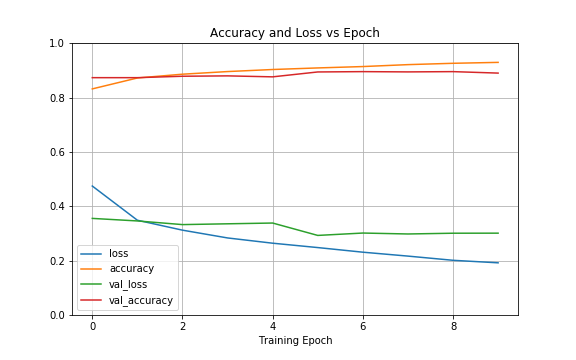
\includegraphics[width = 0.9\textwidth]{hw5/images/acc-p1.png}
    \label{fig:acc1}
    \caption{Training progress for the fully-connected network.}
\end{figure}

\begin{figure}[H]
  \centering
    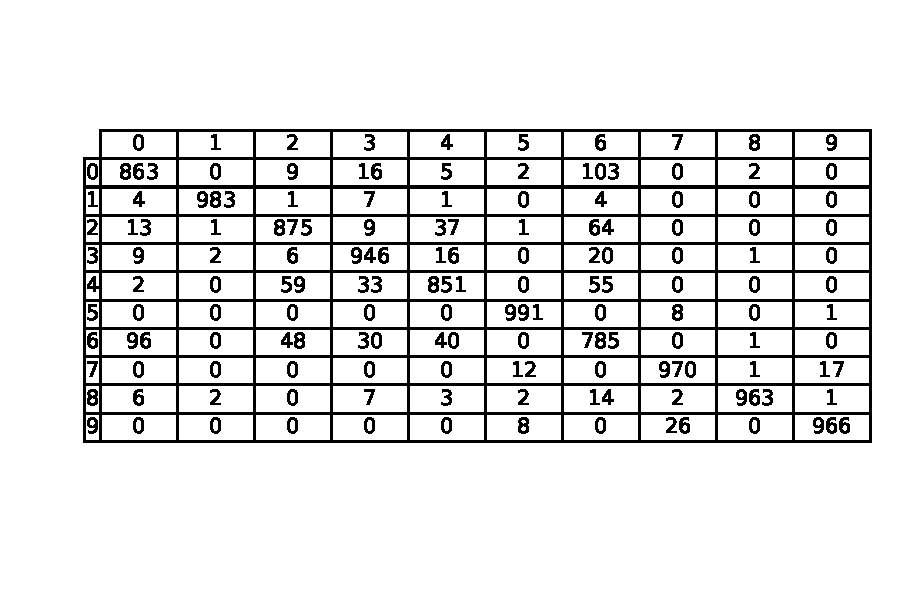
\includegraphics[width = 0.7\textwidth]{hw5/images/conf_mat-p1.pdf}
    \label{fig:conf1}
    \caption{Confusion matrix for the fully-connected network.}
\end{figure}

\begin{figure}[H]
  \centering
    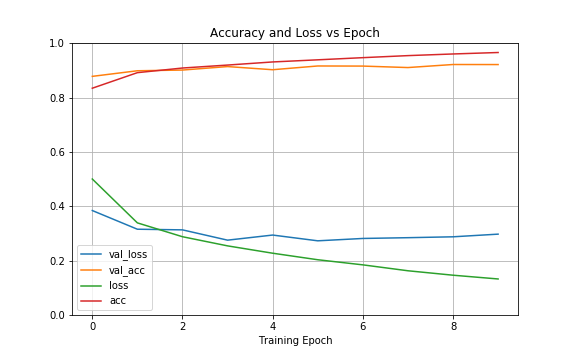
\includegraphics[width = 0.9\textwidth]{hw5/images/acc-p2.png}
    \label{fig:acc2}
    \caption{Training progress for the convolutional network.}
\end{figure}

\begin{figure}[H]
  \centering
    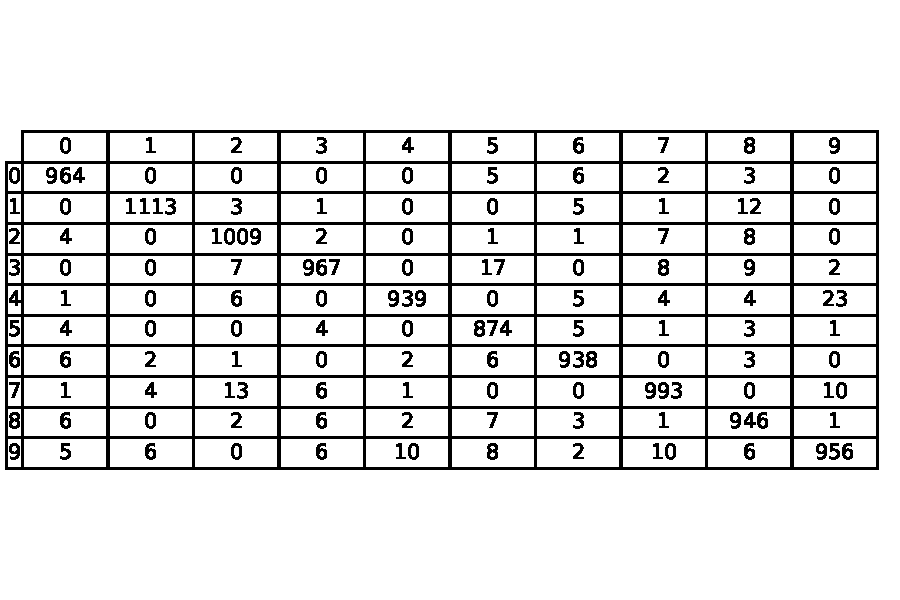
\includegraphics[width = 0.7\textwidth]{hw5/images/conf_mat_p2.pdf}
    \label{fig:conf2}
    \caption{Confusion matrix for the convolutional network.}
\end{figure}


\section{Summary and Conclusions}
Both neural network architectures used in this report displayed powerful results with relatively little computational time or power. Simply to be able to teach a computer to recognize clothing, let alone do it in under a half hour for each model, is incredible. The potential applications for this technology, and for algorithms with complexity and computational demand far beyond the scope of this paper, are nothing short of revolutionary. To be able to harness this computational power, we must explore models and diligently experiment with their design to determine each architecture's strengths, weaknesses, and use cases. On a personal note, what I found most amazing about this technology is the ability to give a computer the power of sight (an exceptionally conscious-creature-like trait, in my opinion) simply with mathematics. The parallel between neural networks and the human brain suggests, at least to me, that humans, too, are imbued by nature with a great measure of mathematical beauty.

\section{Appendix A: Selected Python Functions}
See table \ref{tab:func}.
\begin{table}[]
\begin{tabular}{|l|l|}
\hline
\textbf{Function} & \textbf{Implementation} \\ \hline
functools.partial() & used for partial function application, to make certain arguments default for that call \\ \hline
compile() & configures the model for training, with optimizer, loss function, metrics, etc as given \\ \hline
fit() & trains the model for a fixed number of epochs; other important args: batch\_size \\ \hline
evaluate() & returns the loss value and metrics for the tested model \\ \hline
pd.DataFrame(A).plot() & transforms A into a dataframe, then plots it \\ \hline
predict\_classes() & predicts classes for the input data; this is the classification analogue to predict() \\ \hline
confusion\_matrix() & returns the confusion matrix for the tested model, as described in Computational Results. \\ \hline
\multicolumn{2}{|l|}{\textit{\quad\quad tf.keras.layers}} \\ \hline
Dense() & dense (fully-connected) layer; units, activation, initializers, regularizers, etc. as desired \\ \hline
LeakyReLU() & LeakyReLU activation function, as described in Theoretical Background in this paper \\ \hline
Flatten() & flattens the input but does not otherwise change values \\ \hline
BatchNormalization() & normalizes the activations of the previous layer at each batch \\ \hline
Conv2D() & 2D convolution layer; filters, kernel\_size, strides, padding, activation, etc. as desired \\ \hline
\end{tabular}
\caption{Important Python functions.}
\label{tab:func}
\end{table}
\section{Appendix B: Python Code}
\begin{lstlisting}
## fully connected network
# imports
import numpy as np
import tensorflow as tf
import matplotlib.pyplot as plt
import pandas as pd
from sklearn.metrics import confusion_matrix

fashion_mnist = tf.keras.datasets.fashion_mnist
(X_train_full, y_train_full), (X_test, y_test) = fashion_mnist.load_data()

# split data
X_valid = X_train_full[:5000] / 255.0
X_train = X_train_full[5000:] / 255.0
X_test = X_test / 255.0
y_valid = y_train_full[:5000]
y_train = y_train_full[5000:]

# build model
from functools import partial
dense_layer = partial(tf.keras.layers.Dense, activation=None, kernel_regularizer=tf.keras.regularizers.l2(0.0001))
lrelu = tf.keras.layers.LeakyReLU(alpha=0.1)
bn = tf.keras.layers.BatchNormalization()
model = tf.keras.models.Sequential([
    tf.keras.layers.Flatten(input_shape=[28,28]),
    dense_layer(1024),
    lrelu,
    bn,
    dense_layer(512),
    lrelu,
    tf.keras.layers.BatchNormalization(),
    dense_layer(256),
    lrelu,
    tf.keras.layers.BatchNormalization(),
    dense_layer(10, activation="softmax")
])
model.compile(loss="sparse_categorical_crossentropy",
             optimizer=tf.keras.optimizers.Adam(learning_rate=0.0001),
             metrics=["accuracy"])
             
# run model
history = model.fit(X_train, y_train, epochs=10, validation_data=(X_valid, y_valid))

# evaluate
model.evaluate(X_test,y_test)

# view results
pd.DataFrame(history.history).plot(figsize=(8,5))
plt.grid(True)
plt.gca().set_ylim(0,1)
plt.xlabel('Training Epoch')
plt.title('Accuracy and Loss vs Epoch')
#plt.show()
plt.savefig('acc-p1.png')

y_pred = model.predict_classes(X_test)
conf_test = confusion_matrix(y_test, y_pred)
print(conf_test)

## convolutional network
# imports
y_pred = model.predict_classes(X_test)
conf_test = confusion_matrix(y_test, y_pred)
print(conf_test)

fashion_mnist = tf.keras.datasets.fashion_mnist
(X_train_full, y_train_full), (X_test, y_test) = fashion_mnist.load_data()

# split data
X_valid = X_train_full[:5000] / 255.0
X_train = X_train_full[5000:] / 255.0
X_test = X_test / 255.0
y_valid = y_train_full[:5000]
y_train = y_train_full[5000:]
X_train = X_train[..., np.newaxis]
X_valid = X_valid[..., np.newaxis]
X_test = X_test[..., np.newaxis]

# build model
from functools import partial
my_dense_layer = partial(tf.keras.layers.Dense, kernel_regularizer=tf.keras.regularizers.l2(0.0001))
my_conv_layer = partial(tf.keras.layers.Conv2D, activation="tanh", padding="same")
lrelu = tf.keras.layers.LeakyReLU(alpha=0.1)
model = tf.keras.models.Sequential([
    my_conv_layer(128,5,padding="same",input_shape=[28,28,1]),
    tf.keras.layers.MaxPooling2D(2),
    my_conv_layer(256,5),
    tf.keras.layers.MaxPooling2D(2),
    my_conv_layer(512,5),
    tf.keras.layers.Flatten(),
    my_dense_layer(128),
    lrelu,
    my_dense_layer(64),
    lrelu,
    my_dense_layer(10, activation="softmax")
])
model.compile(loss="sparse_categorical_crossentropy",
             optimizer=tf.keras.optimizers.Adam(lr=0.0001),
             metrics=["accuracy"])

# run model
history = model.fit(X_train, y_train, epochs=10, validation_data=(X_valid,y_valid))

# evaluate
model.evaluate(X_test,y_test)

# view results
pd.DataFrame(history.history).plot(figsize=(8,5))
plt.grid(True)
plt.gca().set_ylim(0,1)
plt.xlabel("Training Epoch")
plt.title("Accuracy and Loss vs Epoch")
plt.show()
plt.savefig('acc-p2.png')

y_pred = model.predict_classes(X_test)
conf_test = confusion_matrix(y_test, y_pred)
print(conf_test)
\end{lstlisting}

\end{document}